%
% Template for Doctoral Theses at Uppsala 
% University. The template is based on    
% the layout and typography used for      
% dissertations in the Acta Universitatis 
% Upsaliensis series                      
% Ver 5.2 - 2012-08-08                  
% Latest version available at:            
%   http://ub.uu.se/thesistemplate            
%                                         
% Support: Wolmar Nyberg Akerstrom        
% Thesis Production           
% Uppsala University Library              
% avhandling@ub.uu.se                          
%                                         
%%%%%%%%%%%%%%%%%%%%%%%%%%%%%%%%%%%%%%%%%%%


\documentclass{UUThesisTemplate}

% Package to determine wether XeTeX is used
\usepackage{ifxetex}

\ifxetex
	% XeTeX specific packages and settings
	% Language, diacritics and hyphenation
	\usepackage[babelshorthands]{polyglossia}
	\setmainlanguage{english}
	\setotherlanguages{swedish}

	% Font settings
	\setmainfont{Times New Roman}
	\setromanfont{Times New Roman}
	\setsansfont{Arial}
	\setmonofont{Courier New}
\else
	% Plain LaTeX specific packages and settings
	% Language, diacritics and hyphenation
    % Use English and Swedish languages. 
	\usepackage[swedish,english]{babel} 

	% Font settings
	\usepackage{type1cm}
	\usepackage[latin1]{inputenc}
	\usepackage[T1]{fontenc}
	\usepackage{mathptmx}
	
	% Enable scaling of images on import
	\usepackage{graphicx}
\fi


% Tables
\usepackage{booktabs}
\usepackage{tabularx}

% *** SUB+FIGURE PACKAGES ***
\usepackage{graphicx}
\usepackage{wrapfig}
\usepackage{float}
%\usepackage[tight,footnotesize]{subfigure}
% http://www.ctan.org/tex-archive/obsolete/macros/latex/contrib/subfigure/
% subfigure.sty has been superceeded by subfig.sty.

%\usepackage[caption=false]{caption}
\usepackage[font=footnotesize]{subfig}
% http://www.ctan.org/tex-archive/macros/latex/contrib/subfig/
% http://www.ctan.org/tex-archive/macros/latex/contrib/caption/

% *** FLOAT PACKAGES ***
\usepackage{fixltx2e}
% http://www.ctan.org/tex-archive/macros/latex/base/

%\usepackage{stfloats}

% *** PDF, URL AND HYPERLINK PACKAGES ***
\usepackage{url}
% http://www.ctan.org/tex-archive/macros/latex/contrib/misc/
% \url{my_url_here}.

%\usepackage{epigraph}
%\epigraphfontsize{\small\itshape}
%\setlength\epigraphwidth{8cm}
%\setlength\epigraphrule{0.5pt}

\makeatletter
\renewcommand{\@chapapp}{}% Not necessary...
\newenvironment{chapquote}[2][2em]
{\setlength{\@tempdima}{#1}%
	\def\chapquote@author{#2}%
	\parshape 1 \@tempdima \dimexpr\textwidth-1\@tempdima\relax%
	\itshape}
{\par\normalfont\hfill--\ \chapquote@author\hspace*{\@tempdima}\par\bigskip}
\makeatother

\usepackage{textcomp}

% Document links and bookmarks
\usepackage{hyperref} 

%bib latin-1 inputenc problem
%\usepackage[latin1]{inputenc}
%\usepackage[bibencoding=utf8]{biblatex}

% Numbering of headings down to the subsection level
\numberingdepth{subsection}

% Including headings down to the subsection level in contents
\contentsdepth{subsection}


% Uncomment to use a custom abstract dummy text
\abstractdummy{
	\begin{abstract}
		This paper proposes a novel power management solution for the resource-constrained devices in the context of Internet of Things (IoT). We focus on smart-phones in the IoT, as they are getting increasingly popular and equipped with strong sensing capabilities. Smart-phones have complex and chaotic asynchronous power consumption incurred by heterogeneous components including their on-board sensors. Their interaction with the cloud can support computation offloading and remote data access via the network. In this work, we aim at monitoring the power consumption behaviours of smart-phones and profiling individual applications and platform to make better decisions in power management. A solution is to design architecture of cloud orchestration as an epic predictor of the behaviours of smart devices with respect to time, location, and context. We design and implement this architecture to provide an integrated cloud-based energy monitoring service. This service enables the monitoring of power consumption on smart-phones and support data analysis on massive data logs collected by large number of users.
	\end{abstract}
}


\begin{document}



\frontmatter

    % Creates the front matter (title page(s), abstract, list of papers)
    % for either a Comprehensive Summary or a Monograph.
    % Authors of Comprehensive Summaries use this front matter 
    \frontmatterCS 
    % Monograph authors use this front matter 
    %\frontmatterMonograph 
    \chapter*{Acknowledgement}
    I thank my supervisor Edith Ngai for her support and for helping me out whenever I have doubts. With the freedom she gave I have excelled and mastered many new skills.
    \addcontentsline{toc}{section}{Acknowledgement}
   % Optional dedication
   \dedication{Dedicated to \\ \ \\  The eyes: \textbf{Wife and Mom} \\ The shoulders: \textbf{Dad and Father-in-law} \\  The arms: \textbf{Brothers and Sisters} \\ Two little stars : \textbf{Charu Nethra , Priyanga} \\ The 'indeed-in-needs' : All my great \textbf{Friends} \\ \& \\ The precious rarities: Motivating \textbf{Relatives} }
 
    % Environment used to create a list of papers
    \begin{listofpapers}
    	\item P. Sathyamoorthy , E.H. Ngai. Energy Efficiency as a Orchestration Service for the Internet of Things. In S. Forsstrom and M. Jacobsson, chairs, \emph{Proceedings of SNCNW 2015, the 11th Swedish National Computer Networking Workshop}, pages 41-44. SNCNW 2015. \label{apaperlabel}
    \end{listofpapers}
    
    
    \begingroup
        % To adjust the indentation in your table of contents, uncomment and enter the widest numbers for each level
        %  E.g.  \settocnumwidth{widest chapter number}{widest section number}{widest subsection number}...{...}
       %  \settocnumwidth{5}{4}{5}{3}{3}{3}
        \tableofcontents
    \endgroup
    
    % Optional tables
    \listoftables
    \listoffigures

\mainmatter
    % This includes the "Instruction", "Problem and Solutions" and "Example" files. After reading it, remove it from Thesis.tex. 
   
    \chapter{Introduction}
%http://eetd.lbl.gov/ee/ee-3.html - who does efficiency?
% Tell policies and other over all big picture
%http://spectrum.ieee.org/computing/hardware/moores-law-might-be-slowing-down-but-not-energy-efficiency
%http://spectrum.ieee.org/tech-talk/computing/hardware/mit-researchers-build-a-100fold-more-efficient-transmitter-
%http://whatis.techtarget.com/definition/Internet-of-Things
%http://www.slideshare.net/IoTMethodology/a-methodology-for-building-the-internet-of-things-42112202?ref=http://www.iotmethodology.com/
%\subsection{The Context of Interest: Smartphones}

\begin{chapquote}{D. Clark,  \textit{End-To-End Arguments in System Design}, 1984}
	``The function in question can completely and correctly be implemented only with
	the knowledge and help of the application standing at the endpoints of the
	communication system. Therefore, providing that questioned function as a feature
	of the communication system itself is not possible. (Sometimes an incomplete
	version of the function provided by the communication system may be useful as a
	performance enhancement.)'' 
\end{chapquote}

%\epigraph{text }{source }

IoT is a convergence of number of technologies such as \textit{sensors}, \textit{IPv6}, \textit{wireless communication} and  \textit{Internet}. Any real-world objects become smart just by satisfying few conditions but not limited to: 1) uniquely identifiable;  2) being able to sense or actuate; 3) being able to communicate \cite{IoT:Defn}. The growth of smart objects are posing challenges to the research community in energy management, data analytics and security \cite{IoT:Challenge}. Among these challenges, security and privacy issues are not just issues in technical system design level, but also in ethical, behavioural and policies level. We have powerful analytical tools available with advanced data analysis algorithms \cite{BigD:Deep}. On the other hand, energy management is more complex and chaotic, that is our focus of this paper. 

%\subsection{Energy Efficiency: The Ins and Outs}
Berkeley National Laboratory defined energy efficiency as using less energy to provide the same service. The need for energy efficiency highly inevitable in almost every type of industries, companies and organizations including Information and Communications Technology (ICT). Energy management in Internet of Things(IoT) aims at reducing the electricity, which is beneficial for many industries to reduce their electricity bills. As the smart objects becoming smaller in size, their small sized batteries provide limited power for operations. Even the smart appliances are idle, they could indirectly waste huge amount of energy in long term and eventually increase the electricity bills too. "Although ICT can enable energy efficiency across all sectors, at present there is little market incentive to ensure that network-enabled devices themselves are energy efficient. In fact, up to 80\% of their electricity consumption is used just to maintain a network connection. While the quantity of electricity used by each device is small, the anticipated massive deployment and widespread use makes the cumulative consumption considerable" as reported by International Energy Agency in \cite{IEA:bdle}.

%\subsection{Energy of Energy Efficiency}
Hereafter we narrow our focus on smart-phones which are increasing in exponential order over the years. Modern smart-phones provide heterogeneous functionalities including a number of sensors. They are one of the most representative and popular smart objects in the IoT. As smart-phones are resource constraint with respect to memory and computation, they happen to off-load computation and access remote storage on the cloud servers via network. Cloud computing in the IoT leads to thousands of cloud supported applications and it is growing steeply. As a consequence, smart-phones are consuming a lot of energy for communication with the cloud. Due to the size limitation, effort of making powerful batteries is not able to withstand the energy hungriness persist in the smart-phones. It is important to reduce energy consumption when developing new kind of applications.

Smart-phones are usually running multiple applications with different operations at the same time. It is very difficult to understand and identify the cause of high energy consumption in this asynchronous power consuming environment. It is necessary to provide profiling of power consumption in at different levels, such as whole system, individual applications, and system calls in operation level. In this paper, we propose the first iterative novel solution using \textit{Cloud Orchestration} for power management on smart-phones. Cloud orchestration aggregates power profiling data from the smart-phones and coordinates data storage, data analysis, learning and decision making. From the profiling data, the orchestrator learns mainly the power consumption behaviours and the usage pattern of the participating smart-phones. The orchestrator aims for providing overall system power management rather than making part of the system efficient. 

{\bf Structure of the chapter.} In this chapter, we first elucidate the ambiguity of the term \emph{energy efficiency} (see Section \ref{section:prob}) and introduce the challenges and the research questions (see Section \ref{section:rq}) that we address in this thesis. Then we discuss the delimitations of the thesis (see Section \ref{section:dlimit}) . In the final section , we give the outline of the rest of this thesis (see Section \ref{section:outln}). 
\section{Energy Efficiency}
\label{section:prob}
The term \emph{energy efficiency} is referred to the way of achieving more services for the same amount of energy, or the same services for less amount of energy, until otherwise specified. Thus the thesis focuses on \textit{efficient energy usage} rather than \textit{energy conversion energy} and \emph{energy conservation} which are commonly confused with energy efficiency. 
Energy conversion efficiency is the ratio between  the useful output of an energy conversion system and the input, in energy terms. Energy conservation refers to reducing energy consumption through using less of an energy service.

Energy efficient communication is only considered as a  constituting disciplinary of \emph{green communications}. However, greenness and optimization of end-to-end communication flow, computing,  the involved intermediate hardwares and other components are overwhelming scopes for this thesis.  We are more towards energy efficiency as software engineering, designed and architect  from data-driven intelligence and thus heavily limited to smart devices(users) and the applications. We also want the architecture to be flexible, adaptable and comprehend to future changes  or optimizations in network layers. Thus by not compromising the improvements made out of domain knowledge.\\
 

\section{Research Questions}
\label{section:rq}
In this section, we elaborate the challenges 

\subsection{Q1: Domain Knowledge} 
Do we have enough domain knowledge to provide a outstanding energy efficient data communications? What are the other factors worth considering ? Why?

\subsection{Q2: Cloud Solutions}
Big data, large scale cloud computing and services, crowd sourcing are new concepts that are aiming to boost data-driven intelligence and insights building. How to integrate these concepts to design a architecture for energy efficiency?

\subsection{Q3: Self Efficiency}
How to ensure the solution for energy efficiency is self energy efficient, i.e., energy consumed by the solution method < the energy it saved ?


%When the architecture, protocols , 
%Question 1: Energy efficiency is really needed?
%Question 2: Does the energy problem breakable into small independent problems?
%Question 3: Does the proposed solution is self energy-efficient?
\section{Delimitations}
\label{section:dlimit}
\section{Outline}
\label{section:outln}



    \chapter{Background}





\section{Theory }
In this section we highlight fundamental concepts and information needed for the thesis.
\subsection{Android : System and Performance Constraints}
%https://source.android.com/source/index.html
%https://source.android.com/compatibility/index.html
%https://android.googlesource.com/platform/frameworks/base/+/master/core/res/res/xml/power_profile.xml
%https://source.android.com/devices/tech/power/index.html#power-values
%https://source.android.com/devices/tech/power/index.html
%http://www.tutorialspoint.com/android/android_architecture.htm
%https://developer.android.com/tools/performance/index.html - important
Android\texttrademark{} is an open source system software stack, built on top of the Linux kernel, that provides services and supports variety of (mobile) devices. Figure \ref{fig:androidstack} shows the Android software stack  and figure  \ref{fig:androidarch} shows the architecture of the Android operating system that are referred by applications developers, hardware developers, Original Equipment Manufactures (OEM) and carriers. This leads to variety of customizations and uncontrolled customization would result in incompatible implementations. Hence, Android tightly integrate OEMs with the \textit{Android Compatibility program}, developers with \emph{Android SDK}, users with \emph{Google Play}. For this thesis only devices with the compatible Android ecosystem is considered.

\begin{figure}[h]	
	\centering
	\includegraphics[width=0.9\textwidth]{Figures/c1framework.png}
	\caption{Android Stack \small(https://source.android.com)}
	 \label{fig:androidstack}
\end{figure} 

\begin{figure}[h]
	\begin{center}	
	\includegraphics[width=0.7\textwidth]{Figures/c1architecture.png}
   \end{center}
	\caption{Android System Architecture \small(https://source.android.com)}
	\label{fig:androidarch}
\end{figure} 

\subsubsection*{Rendering}
This 


\subsection{Energy Profiling}
external, utilization-based, system call level
\subsection{Energy Models}
mathematical
\subsection{Energy Drain Prediction}
\subsection{Crowd Sourcing}
\subsection{Big Data Analysis}
\subsection{Data communications}
\subsection{Cloud Architectures}
Amazon , Google Compute, Heroku
\section{Related Works and Interesting Results}
There has been many efforts made to enable energy efficiency in smart-phones and in IoT in general. They are a range of solutions tried out in \emph{Hardware Architecture} level \cite{EE:MCCarch,EE:JVM}, \emph{Data communication} level \cite{EE:eTime,EE:Multinets},  \emph{Network infrastructure} level \cite{EE:Hier} and in \emph{Protocols} optimization \cite{EE:Protocol}. As Intel summed up in \cite{EE:GreenSW}, \emph{Software Energy Efficiency} is towards achieving \emph{Computational Efficiency}, \emph{Data Efficiency}, \emph{Context Awareness} and \emph{Idle Efficiency} in broader sense. Few common problems with most of the existing solutions are including: 1) system as a whole was not considered;
2) trade-off between components was not properly considered;
3) interdependences of the components was not properly studied;
4) the existing solutions are suboptimal. For measuring energy consumption, solid background has been provided  in \cite{EE:Measure}. Internet of Things-Architecture, a consortium is rigorously developing architectural reference models. The models could potentially serve the best initial  guidance towards concrete architecture for the problem of interest and eventually towards the actual system architecture \cite{IoTA:ARM}. In \cite{Orches:Arch}, devices orchestration is explained in business process point of view.
%%%%%%%%%%%%% Extra %%%%
%\begin{wrapfigure}{l}{0.3\textwidth}
% \begin{center}
%  \includegraphics[scale=0.30]{Figures/IoTArch.png}
% \end{center}
% \caption{IoT Architecture}
%\end{wrapfigure}

%\begin{figure}[H]
% \begin{center}
%  \includegraphics[scale=0.30]{Figures/IoTArch.png}
% \end{center}
% \caption{IoT Architecture}
%\end{figure}

% \cite{EE:Protocol,EE:Hier,EE:RedunData,EE:Diagnosis,
% EE:Measure,EE:MeasureWiFi,EE:Perform,EE:GreenSW,EE:Eaware}
    \input{Sections/method.tex}
    \input{Sections/results.tex}
    \chapter{Conclusions}
\section{Requirements}
\section{Issues}
\section{Future Work}
Orchestrator is in essence the behaviour predictor of the participating devices with respect to time, location and as many as added contexts. The agent application installed in the smart-phones which report logs to the orchestrator will be facilitated with local validator and action triggers which is regularly updated by orchestrator according to the needs to avoid wasting orchestrator energy and data communication for well learnt case. In order to successfully deploy such orchestration service, we need to study and explore all its components defined in the previous section and their interdependencies in detail.  Then we focus on the questions including 1) how to develop low energy consuming profiler? 2) how to reduce logs reporting thus by reduce data communication? 3) how to make orchestrator an epic predictor of device behaviours? 4) how to find optimal responsibilities of local agent by ensuring minimal computation ans resources? 5) Is it best fit for mass open source contribution? 6) What are the de-facto tools for over all implementation? We plan to implement and test the prototype iteratively. This work could be then extended or simplified to other type of IoT devices.
\section{Conclusion}
In this paper we proposed a novel solution for improving energy efficiency in smartphones as a cloud orchestration. We have explained the components of the orchestration and their functionalities. The architecture design is flexible so that new components can be added easily. The \emph{big data}, \emph{knowledge graph}, \emph{control box} will be accessible openly so that mass collaborators can participate and test. It will help improving the orchestrator implicitly or at the least for bug reporting. There is a potential that the big data knowledge would be useful in solving a number of other problems and enabling new services.
   % \chapter{Orchestration}

\section{General Context}
IoT initially had two visions, one is \textit{Internet oriented} vision and another one is \textit{Things oriented} vision. Later when new challenges introduced such as unique addressing and storing information, \emph{Semantic oriented} vision had arisen \cite{IoT:Survey}. According to the orientation, the participating devices are categorised and the orchestration is configured. In smart-phones, all the visions are exists. 
\subsection{IoT elements of smartphones}
In \cite{IoT:Arch}, the general architecture of IoT is well explained as four layers. \emph{Perception Layer} is where all the information collected, say, from the environment using specialised equipments such as sensors and GPS. Thus this layer provides the digital representation of physical world. \emph{Network Layer} is for communication and transmission of information. \emph{Middle-ware Layer} by its various intelligent cloud computing supports the application layer and act as a intermediate between network layer and application layer. \emph{Application Layer} is fully customized with respect to the users and the purpose of the application. In some scenarios, both the perception layer and application layer reside in the same smart-phone system.
\subsection{Need for orchestration}
The main goal is to provide energy efficient decision(s) back to the service enabled smart-phones which are participating in the Orchestration. Orchestration, the concept existing in the music world was adopted in the process automation of business world by automating, coordinating and managing complex systems, middle-wares and services. In the context of vulnerability to energy efficiency, even a single piece of code  ( {\tt while(battery.percentage) println(battery.percentage)}) could be potentially dangerous, leading any effort made to find suboptimal solutions into vain. Hence, there is a need for the great intelligent system, which is capable of finding and categorizing the energy errors. The system should have access to powerful \textit{dynamic control system engine} for fixing such errors. To assist bug fixing we may need a strong insights from the big data of crowd sourced logs/operations  over the time. The big data may lead to \emph{side-effect services} (new enabling services other than energy-efficiency). Hence the energy and effort of making this grant system has huge benefits in return. Thus the \emph{Orchestration}  with the capabilities of integrating different types of clouds, processes and services is an suitable choice. 

\subsection{Composition of systems and models and services}
\begin{figure}[h]
 \begin{center}
 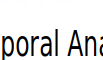
\includegraphics[scale=0.30]{Figures/EEaaOSArchEnhanced.png}
 \end{center}
 \caption{EEaaS Orchestration}
 \label{fig:Orch}
\end{figure}

We propose an architecture design of orchestrator as depicted in Figure \ref{fig:Orch}, with the primary understanding of the participating systems. Then to evaluate and enhance, any existing reference models or relevant solutions in the other related domains may be adopted in the future. The design is open and flexible which make it possible to add,remove and merge number of \textit{systems, models and services} at any granular level in the orchestrator. The orchestrator organizes the following components, \emph{Participating Devices}, \emph{Data Processor}, \emph{Big data storage}, \emph{Knowledge graph}, \emph{Wisdom box}, \emph{Control box} and  \emph{Decision Enhancer} % and \emph{Error Sack}.
\subsubsection{Participating devices}
\label{subsection:partdevice}
These are the devices interested in optimized energy usage. Upon registration with orchestrator, a dark skinned, fully customizable, lower energy consuming background \textit{service application} is enabled in the devices. This application sends low level system-call logs periodically and reports strange system behaviours spontaneously. To avoid security and privacy issues, logs are collected anonymously with unique device profile. This application not only a logs collector, it will also act as local \textit{self-controller}, try to catch energy errors in-time and its functionalities are regularly updated by orchestrator. This is to avoid the need of continuous data communication. 
\subsubsection{Data processor}
Data processor is a collection of APIs for various data processing methods accessible to orchestrator. According to the context, methods will be chosen by the orchestrator. Here the data is processed for both big data analysis and temporal analysis.
\subsubsection{Big data storage and modern tools}
The data produced by smart-phones would be in massive scale over the time. Thus to handle this data-intensiveness we require big data storage and modern cloud programming paradigms such as \emph{Hadoop} and \emph{Apache flink}. For deep analysis of sample data, powerful  computing languages such as \emph{Python} and \emph{R} are required.
\subsubsection{Knowledge graph}
By referring the big data of logs, dynamic knowledge graph is built and then keep on updated. Nodes are qualified classes and subclasses with attribute-value pairs. So it provides a clear and structured view of data. Using this graph, it is then easy to get specific data for analysis with respect to location, device model, internet service provider and for various specification.
% reference is better than saving a copy of graph data 
\subsubsection{Wisdom box}
Wisdom box contains set of learners whose primary focus is building location specific insights (spatial domain). The box act as a predictor of trends in data, usage patterns, system behaviour anomalies. It uses combination of statistical algorithms and machine learning algorithms to find energy efficient decisions. The decisions that are independent of device, platform and applications is stored in \emph{Decision Enhancer} in the orchestration. Device, platform and applications specific decisions fused in the knowledge graph and the reference graph stored in the decision enhancer. 
\subsubsection{Control box}
Control box is a builder of real-time self-controllers for the participating \textit{dynamic systems} with the help of time-sensitive feedbacks (temporal domain). These self-controllers embedded as a service as explained before in \ref{subsection:partdevice}. To make these self-controllers even better, context related decisions in spatial domain are used. Feedbacks are received from the participating devices to evaluate the performance along with log collection.

%% --------Excess -----%
%In this section we would like to highlight some key concepts which is really important to understand our navally proposed cloud orchestration for energy efficiency. First we explain the system architecture of IoT in general and specify that of smartphone . Then the suitable mathematical models from the field of control system theory which deals with dynamic systems.

%fog computing\\
%cloud os\\
%integration of types of clouds\\
%automation\\
%distributed computing

%Internet is constantly evolving phenomenon so is IoT. Hence the problem solver must 
%have best capabilities with respect to the system of devices it deals with including 
%\begin{itemize}
%\item quickly identifies the system
%\item 
%\end{itemize}
%ready to embrace  future changes and flexible. To simply put it , it should have best learning capacity of the system it deals with and  


%Green networking is the practice of selecting energy-efficient networking technologies and products, and minimizing resource use whenever possible.

%https://sites.google.com/site/simulationarchitecture/jeqn
%https://en.wikipedia.org/wiki/Simulink\\

%\subsubsection{Error sack}
%It is in essence reference dictionary of error values for {\tt (input, output)} pairs. For efficiency,the values are received along with next patch of logs. Hence except for the fist time, the participating devices periodically send the logs along with the error values for the previous output signals.
%
%To make the orchestration more efficient, except the participating devices, all other components completely connected thus by improving smartness of the orchestrator to react quickly in case of invalid data inputs and redundancy  and to  achieve some special tasks.
   % \chapter{Results}
% Preliminary investigation and results
\begin{figure}[t]
 \begin{center}
\subfloat[Google maps\label{subfig:gmap}]{ 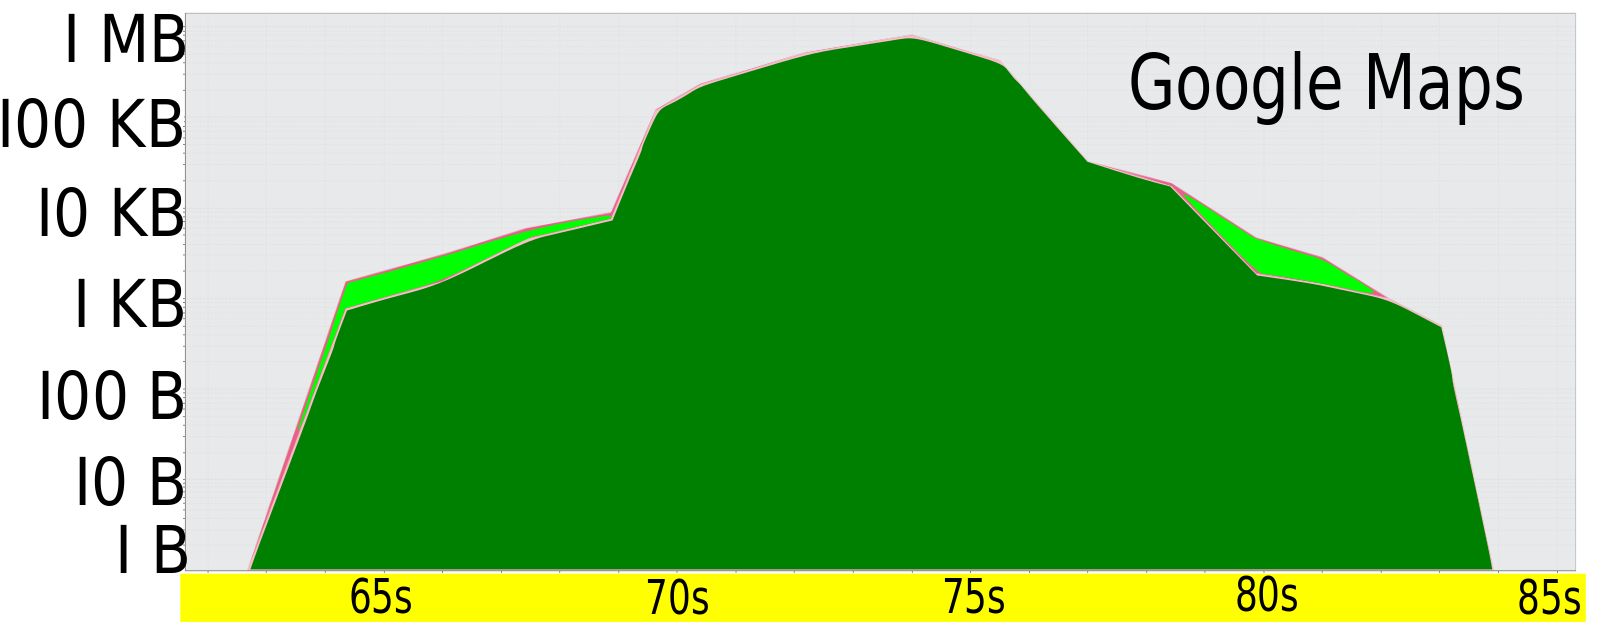
\includegraphics[scale=0.15]{Figures/gmapgps60to80c.png}}
\subfloat[YouTube\label{subfig:ytube}]{ 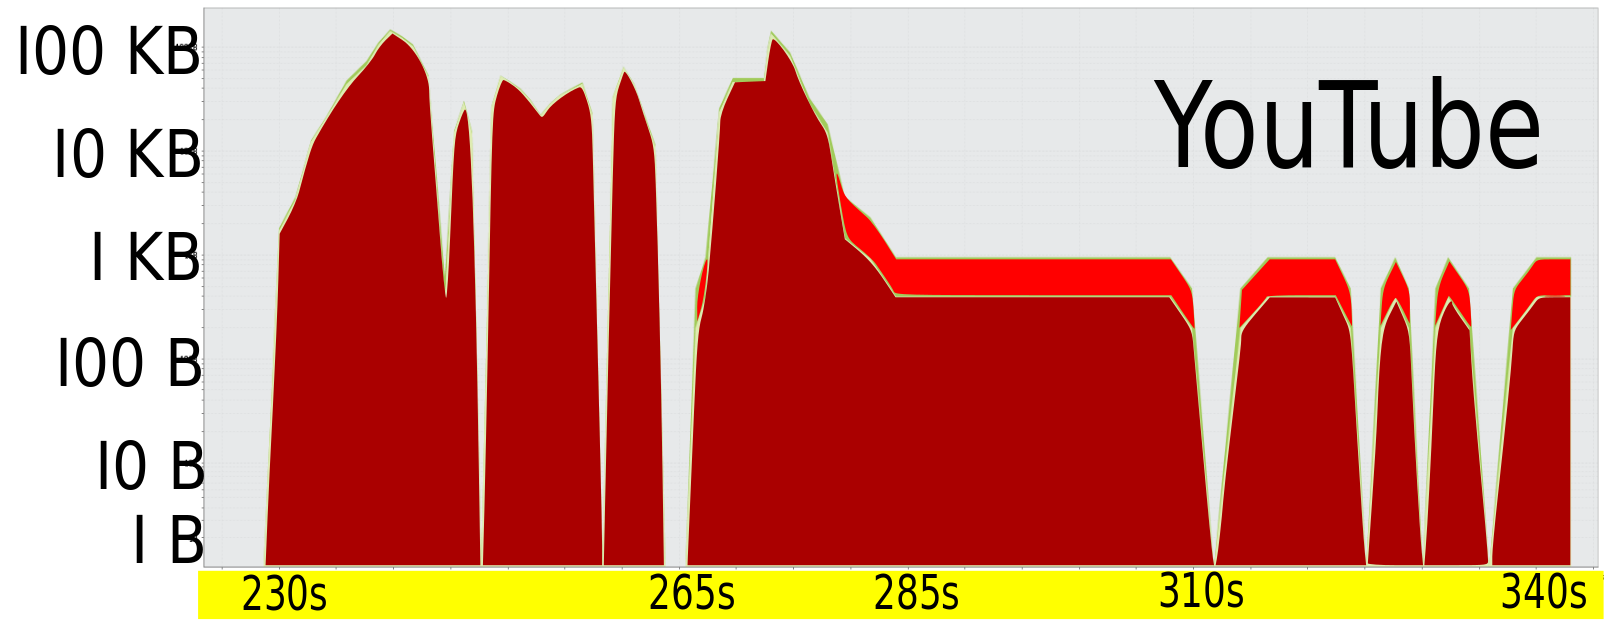
\includegraphics[scale=0.15]{Figures/Youtube230c.png}}
 \end{center}
 \caption{Randomly profiled data usage patterns}
 \label{fig:TrepnDataUsage}
\end{figure} 
Smart-phone is a system-on-chip architecture with three key components  \emph{Application processor} to handle user applications, \emph{Modem processor} to handle transmission and reception and \emph{Peripheral devices(I/O)} to interact with users. In smart-phones, power consumption of any I/O component is sometime higher than the power consumption of the CPU or at the least comparable. In \cite{EModel} the problems and flaws in the power models derived from external power meters and those derived from (hardware) utilization-based well explained by considering the types of components having \textit{tail power states},  not having quantitative utilization(e.g. camera on/off) and system calls that change power states but not mean any utilization of hardware. As system calls are the only way for application can use I/O components, system call based power modelling is better one. Thus Energy profiling with all its overheads is the very important first step.
\subsection{Power states,logging and semantic data}
The Advanced Configuration and Power Interface(ACPI) specification has been evolving as a de-facto common hardware interfaces in Operating System-directed configuration and  Power Management(OSPM) for both devices and entire systems. When profiling either an individual application or entire platform it is useful to fetch information about the states of system, device and processors, as in table \ref{table:states}, so that better decision can be made to achieve energy efficiency. We are currently using Qualcomm's Trepn Profiler \cite{trepn}. We study the behaviours of the system and applications running in the system including CPUs usage, memory usage, data usage. 
\begin{table}[h]
\begin{tabular}{|l|l|l|}
\hline
Global System States & Device Power States  & Processor Power States \\
\hline
G0 Working & D0 - Fully-On  & C0\\
G1 Sleeping & D1  & C1\\
G2/S5 Soft Off & D2 & C2\\
G3 Mechanical Off & D3hot & C3\\
& D3 - Off & \\
\hline
\end{tabular}
\caption{ACPI/OSPM defined power states}
\label{table:states}
\end{table}

As data communication is one of the main reasons for the quicker energy drain in the smart-phones, it is interesting example to profile the data usage patterns of the different applications. In figure \ref{fig:TrepnDataUsage}, profiled data usage patterns of two applications, namely, \textit{Google Maps} and \textit{YouTube} is shown. While profiling google maps, GPS was turned ON at 20th second, maps were zoomed-in and then the device is navigated in random direction. We observed as shown in figure \ref{subfig:gmap}, sudden high usage of data occurred about 10 seconds in the time interval [70, 80]. In this manual profiling and inspection, it is inferred that action of zooming-in the map is the reason for high data usage. Does the state of the GPS being ON has any effect on data usage? The answer seems \emph{no} because of the fact that the GPS is turned ON at 20th second already. If the device lay in the fixed position, the above question doesn't make sense. If the device is in navigation, then it requires fine-tuned profiling again. While profiling youtube, a video is randomly picked for playing, after few seconds the screen is rotated to play the video in full screen mode, the video is continued to play. We observed as shown in figure \ref{subfig:ytube}, the initial aggressive data communications due to pre-fetching. 
These scenario implies: 
\begin{itemize}
\item Usage of resources such as CPU, Memory, GPU and Data varies with respect to applications
\item Weighted effect on energy usage with respected to the resources should be studied
\item Fine-grained profiling is data-intensive and computations-intensive
\item Profiler should be self-energy efficient
\item Automation of profiling with added semantics is extremely challenging
\item Detailed study of interdependencies and contexts is required
\item Mobile cloud computing is suitable
\end{itemize}

We are developing R computing language configured cloud application \emph{EnergyApp} to develop and test energy models and visualize the insights on sample data. The application right now manually let the user to inspect the data collected by Trepn profiler. It also shows simple interactive plots where one can compare the parameters for example, as CPU usage against memory usage for the applications. We further investigate with statistical data analysis and machine learning algorithms. Then we model the smart-phones as dynamic systems as in control systems to develop self-controllers for the participating systems. Then set of data preprocessing methods will be implemented. Then knowledge graph building process will take place. After this phase assembling orchestration will take place. 
\subsection{Future Work}
Orchestrator is in essence the behaviour predictor of the participating devices with respect to time, location and as many as added contexts. The agent application installed in the smart-phones which report logs to the orchestrator will be facilitated with local validator and action triggers which is regularly updated by orchestrator according to the needs to avoid wasting orchestrator energy and data communication for well learnt case. In order to successfully deploy such orchestration service, we need to study and explore all its components defined in the previous section and their interdependencies in detail.  Then we focus on the questions including 1) how to develop low energy consuming profiler? 2) how to reduce logs reporting thus by reduce data communication? 3) how to make orchestrator an epic predictor of device behaviours? 4) how to find optimal responsibilities of local agent by ensuring minimal computation ans resources? 5) Is it best fit for mass open source contribution? 6) What are the de-facto tools for over all implementation? We plan to implement and test the prototype iteratively. This work could be then extended or simplified to other type of IoT devices.





%https://en.wikipedia.org/wiki/Advanced_Configuration_and_Power_Interface
%The data is produced either by collecting real data by participatory sensing or by simulation in case of limited availability of real data or in case of testing. 

% Excesss ---- %

%From a power management perspective, OSPM/ACPI promotes the concept that systems should conserve
%energy by transitioning unused devices into lower power states including placing the entire system in a low-power state (sleeping state) when possible.

%\State $syslog \gets \{err, data\}$

%
%Control theory concept to be explained by considering smartphones as dynamic systems( applications and processes = linear/non-linear time/frequency domain signals )
%The above fig is demo, final version may change
%\begin{algorithm}                      % enter the algorithm environment
%\caption{Generating Energy Efficient Decision Signals }          % give the algorithm a caption
%\label{alg1}                           % and a label for \ref{} commands later in the document
%\begin{algorithmic}                    % enter the algorithmic environment
%	\Procedure{EnableEnergyEfficiency}{}
%    \REQUIRE System-call logs
%    \ENSURE Energy Efficient Decision Signals
%    \STATE $syslog \Leftarrow \{err:\{\}, data:\{\}\}$ % $\#h$
%    \IF{$n < 0$}
%        \STATE $X \Leftarrow 1 / x$
%        \STATE $N \Leftarrow -n$
%    \ELSE
%        \STATE $X \Leftarrow x$
%        \STATE $N \Leftarrow n$
%    \ENDIF
%    \WHILE{$N \neq 0$}
%        \IF{$N$ is even}
%            \STATE $X \Leftarrow X \times X$
%            \STATE $N \Leftarrow N / 2$
%        \ELSE[$N$ is odd]
%            \STATE $y \Leftarrow y \times X$
%            \STATE $N \Leftarrow N - 1$
%        \ENDIF
%    \ENDWHILE
%    \EndProcedure
%\end{algorithmic}
%\end{algorithm}

%\State $i \gets \textit{patlen}$
%\BState \emph{top}:
%\If {$i > \textit{stringlen}$} \Return false
%\EndIf
%\State $j \gets \textit{patlen}$
%\BState \emph{loop}:
%\If {$\textit{string}(i) = \textit{path}(j)$}
%\State $j \gets j-1$.
%\State $i \gets i-1$.
%\State \textbf{goto} \emph{loop}.
%\State \textbf{close};
%\EndIf
%\State $i \gets i+\max(\textit{delta}_1(\textit{string}(i)),\textit{delta}_2(j))$.
%\State \textbf{goto} \emph{top}.
%
%\Procedure{Init}{init}
%\State $err \gets \{\}$
%\State $data \gets \{\}$
%\EndProcedure


%\begin{algorithm}
%\caption{Generating Energy Efficient Decision Signals}\label{eeeff}
%\begin{algorithmic}
%\Require System-call logs
%\Ensure Energy Efficient Decision Signals
%
%\MVAt Devices
%\Procedure{RegisterRequest}{device\_id}
%\EndProcedure
%
%\Procedure{SendLogAndError}{device\_id,err,data}
%\EndProcedure
%
%\MVAt Orchestrator
%\Procedure{RegisterDevice}{device\_id}
%\EndProcedure
%
%\Procedure{EnableEnergyEfficiency}{}
%%\State $syslog \gets \{err, data\}$
%\EndProcedure
%
%\end{algorithmic}
%\end{algorithm}



%\subsection{Inside the control box}
%discussion about 1)Time vs Frequency Domain signals 2) Laplace/ Fourier Transforms 
%\subsection{Data analysis}
%Find the categories and interested questions


%\begin{figure}[H]
% \begin{center}
% \includegraphics[scale=0.45]{Figures/mobilearch1.png}
% \end{center}
% \caption{ARM Architecture(courtesy:www.arm.com)}
%\end{figure} 
    %\input{Example/ProblemsAndSolutions}
    %\input{Example/Example.tex}
    
    % Include your chapters here.
    %\input{Introduction.tex}


\backmatter
    % References
    \begin{thebibliography}{9}    
    	\bibitem{android:evol}
Chandnani, P., \& Wadhvani, R. . “Evolution of Android and its Impact on Mobile Application Development. International Journal of Scientific Engineering and Technology”  1(1), 80–85 ,  2012.


\bibitem{IoT:Defn}
J. Gubbi, R. Buyya, S. Marusic, and M. Palaniswami, “Internet of Things (IoT): A vision, architectural elements, and future directions,” Future Generation Computer Systems, vol. 29, no. 7, pp. 1645–1660, Sep. 2013.
\bibitem{IoT:Challenge}
J. Chase, The Evolution of the Internet of Things. Dallas, TX: Texas Instruments Incorporated, 2013.
\bibitem{BigD:Deep}
M. M. Najafabadi, F. Villanustre, T. M. Khoshgoftaar, N. Seliya, R. Wald, and E. Muharemagic, “Deep learning applications and challenges in big data analytics,” Journal of Big Data, vol. 2, no. 1, Feb. 2015.

\bibitem{IEA:bdle}
International Energy Agency, "More Data, Less Energy - Making Network Standby More Efficient in Billions of Connected Devices" \copyright OECD/IEA, 2014 Licence:\url{https://www.iea.org/t&c/termsandconditions/}

\bibitem{EE:MCCarch}
A. Tzanakaki, M. P. Anastasopoulos, S. Peng, B. Rofoee, Y. Yan, D. Simeonidou, G. Landi, G. Bernini, N. Ciulli, J. F. Riera, and others, “A converged network architecture for energy efficient mobile cloud computing,” in Optical Network Design and Modeling, 2014 International Conference on, 2014, pp. 120–125.

\bibitem{EE:JVM}
T. K. Kundu and K. Paul, “Improving Android Performance and Energy Efficiency,” 2011, pp. 256–261.

\bibitem{EE:eTime}
P. Shu, F. Liu, H. Jin, M. Chen, F. Wen, and Y. Qu, “eTime: energy-efficient transmission between cloud and mobile devices,” in INFOCOM, 2013 Proceedings IEEE, 2013, pp. 195–199.

\bibitem{EE:Multinets}
S. Nirjon, A. Nicoara, C.-H. Hsu, J. Singh, and J. Stankovic, “Multinets: Policy oriented real-time switching of wireless interfaces on mobile devices,” in Real-Time and Embedded Technology and Applications Symposium (RTAS), 2012 IEEE 18th, 2012, pp. 251–260.

\bibitem{EE:Hier}
J. Tang, Z. Zhou, J. Niu, and Q. Wang, “An energy efficient hierarchical clustering index tree for facilitating time-correlated region queries in the Internet of Things,” Journal of Network and Computer Applications, vol. 40, pp. 1–11, Apr. 2014.

\bibitem{EE:Protocol}
A. Venčkauskas, N. Jusas, E. Kazanavičius, and V. Štuikys, “An Energy Efficient Protocol For The Internet Of Things,” Journal of Electrical Engineering, vol. 66, no. 1, pp. 47–52, 2015.

\bibitem{EE:GreenSW}
B. Steigerwald and A. Agrawal, “Developing green software,” Intel White Paper, vol. 9, 2011.

\bibitem{EE:Measure}
A. Pathak, Y. C. Hu, and M. Zhang, “Where is the energy spent inside my app?: fine grained energy accounting on smartphones with eprof,” in Proceedings of the 7th ACM european conference on Computer Systems, 2012, pp. 29–42.

\bibitem{IoTA:ARM}
R. Beneficiary, I. M. L. FhG, S. H. SAP, E. H. HSG, C. Jardak, A. O. CEA, A. Serbanati, M. T. SAP, and J. W. Walewski, “Internet of Things-Architecture IoT-A Deliverable D1. 3–Updated reference model for IoT v1. 5.”
\bibitem{Orches:Arch}
A. González García, M. Alvarez Alvarez, J. Pascual Espada, O. Sanjuán Martínez, J. M. Cueva Lovelle, and C. Pelayo G-Bustelo, “Introduction to Devices Orchestration in Internet of Things Using SBPMN,” International Journal of Interactive Multimedia and Artificial Intelligence, vol. 1, no. 4, p. 16, 2011.

\bibitem{IoT:Survey}
L. Atzori, A. Iera, and G. Morabito, “The Internet of Things: A survey,” Computer Networks, vol. 54, no. 15, pp. 2787–2805, Oct. 2010.
\bibitem{IoT:Arch}
H. Suo, J. Wan, C. Zou, and J. Liu, “Security in the Internet of Things: A Review,” 2012, pp. 648–651.
\bibitem{EModel}
A. Pathak, Y. C. Hu, M. Zhang, P. Bahl, and Y.-M. Wang, “Fine-grained power modeling for smartphones using system call tracing,” in Proceedings of the sixth conference on Computer systems, 2011, pp. 153–168.
\bibitem{trepn}
Qualcomm Technologies, Inc. "Trepn Profiler" \url{https://developer.qualcomm.com/mobile-development/increase-app-performance/trepn-profiler}, Apr. 15, 2015.
    \end{thebibliography}
    
    % No restriction is set to the reference styles
    % Save your references in References.bib
    %\nocite{*} % Remove this for your own citations
    %\bibliographystyle{plain}
    %\bibliography{References}

\end{document}